\documentclass[12pt,titlepage]{article}

%\usepackage{showframe}
\usepackage[a4paper, nomarginpar, left=2.5cm, right=1.5cm,top=2cm, bottom=2cm, total={210mm, 297mm}]{geometry}
\usepackage[utf8]{inputenc}
\usepackage[L7x]{fontenc}
\usepackage[Lithuanian]{babel}
\usepackage{tgtermes}
\usepackage{graphicx}
\usepackage{float}
\usepackage[
backend=biber,
style=apa,
url=false,
sorting=nyt]{biblatex}
\addbibresource{references.bib}
\usepackage{setspace}
\onehalfspacing
\usepackage{hyperref}
\hypersetup{colorlinks=true, linkcolor=black,filecolor=blue, urlcolor=blue,citecolor=blue}
\usepackage{ragged2e}
\usepackage{titlepic}
\usepackage{multirow}

\titlepic{\centering
\includegraphics[scale=1.2]{vu}}
\title{\textbf{Lojalumas prekės ženklui}} 
\author{\textbf{Viktorija Navickaitė}} 



\begin{document}
\maketitle
\tableofcontents
\newpage

\section{Įvadas}

\justify
\hspace{\parindent} Aršios konkurencijos sąlygomis, net ir gerai žinomos įmonės susiduria su pakankamai sudėtinga problema: kaip išsaugoti turimą rinkos dalį ir pasiekti, kad įmonės veikla ir toliau išliktų efektyvi. Įprastai, tokiu atveju, įmonės vadovai nusprendžia imtis tam tikrų priemonių. Pavyzdžiui, mažinti gamybos kaštus ir didinti įmonės užimamą dalį rinkoje, siekiant konkuruoti kainomis. Tačiau tokių sprendimų ne visada pakanka.Labai  svarbu yra rinkodaros specialistams sėkmingai suprasti, kodėl ir kaip vartotojai elgiasi. Ištirti jų elgesį skatinančius veiksnius, kurie turi įtakos vartotojų pirkimų elgesiui. Tad galima teigti, jog įmonių sėkmę lemia ir vartotojų lojalumas prekiniam ženklui.\\

Šiandien prekinis ženklas yra vienas iš svarbiausių nematerialaus turto, kurį bendrovė turi. Sekdami tendencijas pramonėje, galima matyti, kad labai sudėtingoje rinkoje vartotojai daugiausia mėgsta savo išbandytas ir patikimas įmones. Simbolinė prekės ženklo vertė padeda žmonėms pasirinkti geriausią prekės ženklą, kad patenkintų savo poreikius.\parencite{alamgir2011influence} Vartotojai tenkindami savo poreikius dažniausiai perka tą patį prekės ženklą ir į kitus nekreipia dėmesio ir taip parodo savo lojalumą tam prekės ženklui. Tad lojalumas tampa svarbiu konkurenciniu pranašumu, kuris lemia geresnę įmonės padėtį rinkoje ir užtikrina paklausą. Įmonės gali sėkmingai konkuruoti rinkoje ir gauti didesnį pelną.\\

Tačiau svarbu nepamiršti, jog kiekvienai įmonei svarbu stebėti savo vartotojus, pastebėti jų elgesio pakitimus, kad laiku būtų imtasi tinkamų priemonių. Vartotojai pastaruoju metu rinkoje turi daug galimybių rinktis, tad konkurentui pateikus patrauklesnį pasiūlymą, jie gali bet kada atsisakyti savo lojalumo ir pakeisti naudojamą prekės ženklą kitu.  Šiai problemai spręsti, gali padėti empirinis tyrimas, kurio rezultatai gali padėti išsiaiškinti problemines sritis prekės ženklo lojalumo kūrime, tai leistų išsaugoti esamus klientus bei padidinti jų lojalumą, naudojant klientams svarbiausias prekės ženklui skatinančias priemones. Atlikta gautų duomenų analizė, leis geriau suprasti lojalumą prekės ženklui lemiančius veiksnius.
\justify

\section{Prekinis ženklas:}
\subsection{Prekinio ženklo samprata}
\justify
\hspace{\parindent} 
Pažymėtina, kad Lietuvos Respublikos prekių ženklų \href{https://e-seimas.lrs.lt/portal/legalAct/lt/TAD/TAIS.111762?jfwid=tu0odnqqe}{įstatymas} sutaria, jog prekės ženklas – tai pavadinimas, ženklas, simbolis, pakuotė, vardas, emblema, etiketė, devizas (spalva, forma, dizainas) arba jų derinys, naudojami atpažinti vieno pardavėjo ar jų grupės siūlomoms prekėms ir/arba paslaugoms atskirti nuo konkurentų paslaugų ar prekių. Beje, Lietuvos Respublikos prekių ženklų įstatymas pažymi, kad jis nustatyta tvarka užregistruotas ir teisiškai saugomas prekės žymuo.\parencite{vanagiene2008prekes}  Jis tampa firmos intelektualia nuosavybe ir yra galimybė su šio ženklo naudojimu susijusius konfliktus spręsti per teismą.\\

Aptikus bei išskyrus tą vienintelį ypatingą bruožą ar idėją, galima sukurti nepakartojamą prekės ženklą, kuris padės klientui užmegzti emocinį ryšį tarp prekės ženklo ir prekės. Todėl mokslininkai skiria ir emocinį prekės ženklo aspektą, teigdami, kad šis atsispindi vartotojų sąmonėje turi įtakos jų prekės ženklo suvokimui. Anot D. Aleliūnaitės, R. Urbanskienės (2000), prekės ženklo atliekama vertės funkcija – išskirtinės prekės savybės, susiformavusios vartotojo sąmonėje bei suteikiančios papildomą vertę prekei.\\

Apibendrintai galima teigti, jog prekės ženklas – tai apčiuopiamų (pavadinimas, sąvoka, frazė, ženklas, simbolis ir kt.) ir neapčiuopiamų (išskirtinės prekės savybės, vertė ir kt.) elementų derinys, užregistruotas ir teisiškai saugomas prekės žymuo, kuriantis vertę vartotojui ir įmonei. 

\justify

\subsection{Prekinio ženklo vertė}
\justify
\hspace{\parindent}
Prekės ženklo vertė – svarbi koncepcija verslo praktikoje, nes taip kompanijos gali įgyti konkurencinį pranašumą tarp kitų stiprių prekės ženklų. Stiprus prekės ženklas turi solidžią savo vertę. Prekės ženklo vertę lemia vartotojo lojalumas prekės ženklui, prekės pavadinimo paplitimas, suvokiama kokybė, su preke susijusios asociacijos ir kitos vertybės. Turintis didelę vertę prekės ženklas yra reikšmingas bendrovės turtas išliekantis gerokai ilgiau negu konkretūs produktai ar pati bendrovė. Kiekvienas populiarus prekės ženklas turi ištikimus vartotojus. Todėl pagrindinis turtas, lemiantis prekės ženklo vertę, yra vartotojų vertė. Tai reiškia, jog planuojant rinkodaros strategiją daugiausia reikia orientuotis į tai, kad būtų padidinta lojalaus vartotojo per visą jo gyvenimą sukuriama vertė, o prekės ženklo vadyba čia turi tapti pagrindiniu rinkodaros įrankiu.\\

Siekdami išsaugoti prekės ženklo vertę, rinkodaros specialistai privalo atidžiai tuo rūpintis. Jie turi bendradarbiauti su tyrimų ir diegimo padalinio darbuotojais, kad nuolatos būtų pateikiami patobulinti ir naujoviški produktai, kurie patenkintų besikeičiančius klientų poreikius. Šitaip darant daugiau vartotojų sužinos apie prekės ženklą, susidarys gerą nuomonę apie jo kokybę ir naudingumą bei suformuos teigiamas asociacijas.Tad prekės ženklo vertė siūloma matuoti vartotojų požiūriu ir įtraukiant šiuos elementus: prekės ženklo žinomumą, asociacijas ir tikėjimą bei požiūrį ir jausmą. Kiekvienas iš šių elementų gali nusakyti prekės ženklo stiprumą kitų konkurencinių prekės ženklų požiūriu. \parencite{vanagiene2008prekes}\\

Apibendrinant prekės ženklo vertės sąvokos sampratą, tai konkurencinėje kovoje prekės ženklas yra didžiausias ir labiausiai vertinamas turtas, kurį gali turėti kompanija. Stiprūs prekės ženklai turi vertę, kuri turi įtakos vartotojo lojalumui prekės ženklui, suvokiamai kokybei, asociacijoms susijusioms su produktu. Kai prekės ženklu pasitikima, įmonei paprasčiau plėsti asortimentą. Svarbiausia yra tai, kad, turėdama populiarų prekės ženklą, įmonė gali apsiginti nuo negailestingos kainų konkurencijos. \parencite{vanagiene2008prekes}

\justify
\section{Vartotojų lojalumas prekiniam ženklui:}
\subsection{Lojalumo samprata ir jo įvertinimas}
\justify
\hspace{\parindent} 
Vartotojų lojalumas, kaip ilgalaikių santykių tarp organizacijos ir vartotojų pagrindas, ypatingą svarbą įgauna rinkų prisotinimo atveju, kuomet nelieka naujų galimybių rinkos augimui bei išplėtimui. Brandžiose rinkose vartotojų lojalumą pasiekti tampa vis sunkiau: stiprėjanti konkurencija, didėjantis pasirinkimas ir augantis vartotojų išrankumas verčia ieškoti naujų būdų, padedančių išlikti rinkoje ir išlaikyti savo vartotojus.\parencite{zikiene2010vartotojku}\\

Lojalumo koncepcijos užuomazgos siejamos su XX a. penktuoju dešimtmečiu. Literatūroje yra daug lojalumo apibrėžimų. Paprastai rinkodaros literatūroje lojalumas yra apibrėžiamas kaip pakartotinis pirkimo dažnis arba santykinis to paties prekės ženklo pirkimo apimtis.\parencite{oliver1999whence} Patys vartotojai save lojaliais laiko tada, kai iš produktų / paslaugų teikėjų gauna tokią naudą ir patiria tokį pasitenkinimą, kad neieško kito pasirinkimo alternatyvo ir lieka ištikimi vienai produktus / paslaugas teikiančiai firmai.\\

\justify

\begin{table}[H]
\center
\begin{tabular}{|l|c|c|c|c|llll}
\cline{1-5}
\begin{tabular}[c]{@{}l@{}}Stadijos pavadinimas\\ \\  Požymiai\end{tabular}          & \begin{tabular}[c]{@{}c@{}}1 stadija \\ Neutralus\end{tabular} & \begin{tabular}[c]{@{}c@{}}2 stadija \\ Potencialiai \\ lojalus\end{tabular} & \begin{tabular}[c]{@{}c@{}}3 stadija\\  Nesąmoningai\\ lojalus\end{tabular} & \begin{tabular}[c]{@{}c@{}}4 stadija\\  Nuoširdžiai\\  lojalus\end{tabular} &  &  &  &  \\ \cline{1-5}
Elgsena                                                                              & \begin{tabular}[c]{@{}c@{}}Nėra \\ vartojęs\end{tabular}       & \begin{tabular}[c]{@{}c@{}}Perka pirmą\\  kartą\end{tabular}                 & \begin{tabular}[c]{@{}c@{}}Yra pirkęs\\   pakartotinai\end{tabular}         & \begin{tabular}[c]{@{}c@{}}Perka\\   pastoviai\end{tabular}                 &  &  &  &  \\ \cline{1-5}
Alternatyvų paieška                                                                  & Maksimali                                                      & Vidutinė                                                                     & \begin{tabular}[c]{@{}c@{}}Keletas \\ alternatyvų\end{tabular}              & Minimali                                                                    &  &  &  &  \\ \cline{1-5}
Nuostata                                                                             & \begin{tabular}[c]{@{}c@{}}Jokios \\ nuostatos\end{tabular}    & \begin{tabular}[c]{@{}c@{}}Turi galimybę\\  susidaryti nuostatą\end{tabular} & \begin{tabular}[c]{@{}c@{}}Silpna\\  nuostata\end{tabular}                  & \begin{tabular}[c]{@{}c@{}}Pastovi \\ nuostata\end{tabular}                 &  &  &  &  \\ \cline{1-5}
\begin{tabular}[c]{@{}l@{}}Organizacijos galimybės \\ paveikti nuostatą\end{tabular} & \multicolumn{2}{c|}{Sunkiai paveikiama}                                                                                                       & \multicolumn{2}{c|}{Lengvai paveikiama}                                                                                                                   &  &  &  &  \\ \cline{1-5}
\begin{tabular}[c]{@{}l@{}}Konkurentų galimybės \\ paveikti nuostatą\end{tabular}    & \multicolumn{2}{c|}{Lengvai paveikiama}                                                                                                       & \multicolumn{2}{c|}{Sunkiai paveikiama}                                                                                                                   &  &  &  &  \\ \cline{1-5}
Marketingo orientacija                                                               & \multicolumn{2}{c|}{Tradicinis marketingas}                                                                                                   & \multicolumn{2}{c|}{Ryšių marketingas}                                                                                                                    &  &  &  &  \\ \cline{1-5}
\end{tabular}
\caption{Vartotojų lojalumo stadijos}
\label{tab:table1}
\end{table}

\justify
\hspace{\parindent}
Žmonės lojaliais vartotojais tampa palaipsniui. Tai procesas, susidedantis iš kelių stadijų. Visi vartotojai, remiantis jų nuostatų ir elgsenos prekės ženklo (produkto/ paslaugos/ parduotuvės) atžvilgiu charakteristikomis, gali būti priskirti tam tikrai lojalumo stadijai – (1) „Neutraliems“, (2) „Potencialiai lojaliems“, (3) „Nesąmoningai lojaliems“ ir (4) „Nuoširdžiai lojaliems“ (\ref{tab:table1} lentelė). Vartotojai, pasiekę skirtingas lojalumo stadijas, turi nevienodus poreikius. Minėtų stadijų atpažinimas ir specifinių poreikių patenkinimas organizacijai suteikia daugiau galimybių, formuojant vartotojų lojalumą. Vartotojų lojalumo formavimui galima naudoti tam tikrą atlygį vartotojams – pardavimų skatinimą. Pardavimų skatinimas turi būti planuojamas, derinant su lojalumo stadija, kurią yra pasiekęs vartotojas. Žinodama kiekvienai lojalumo stadijai priskiriamų vartotojų charakteristikas bei poreikius, organizacija gali planuoti bei naudoti tokį pardavimų skatinimą, kuris tiksliau atitiks individualaus vartotojo poreikius. \parencite{pileliene2008pardavimku}
\justify
\subsection{Vartotojų lojalumas rinkodaros srityje}
\justify
\hspace{\parindent}
Vartotojų lojalumas yra viena reikšmingiausių šiuolaikinių strategijų, padedanti užtikrinti ne tik įmonės verslo sėkmę, bet ir ilgalaikiuose vartotojo bei įmonės santykiuose, palaikant ir stiprinant vartotojų lojalumą gauti naudos abiem šalims. Įmonei lojalius vartotojus yra pigiau išlaikyti ir aptarnauti.  Lojalūs vartotojai yra mažiau jautrūs kainai, atlieka reklaminę funkciją, perduoda informaciją bei teigiamas rekomendacijas „iš lūpų į lūpas", daugiau ir dažniau įsigyja prekių /paslaugų, papildomų produktų, yra imlesni naujiems pasiūlymams.  Tuo tarpu lojalūs vartotojai jaučia mažesnę riziką, didesnį pasitikėjimą įmone ir pasitenkinimą teikiančių įsigyjamų produktų, o ilgalaikiai santykiai su įmone suteikia išskirtinumo pojūtį. \\

Klientų lojalumo programos kūrimas gali suteikti galimybę ilgiau išlaikyti pirkėjus ir su jais palaikyti ilgalaikius santykius, tačiau dažnai neatsižvelgiama į tai, kokią apčiuopiamą finansinę naudą ši programa įmonei gali duoti. Įmonės lojalumo programos kartais vertinamos tiesiog kaip reklaminės akcijos, kurios padeda trumpam padidinti pardavimų skaičių. \parencite{vzigiene2006lojalumo} Toks vertinimas nėra tikslus, nes lojalumo programa gali atsipirkti tik per ilgą laiką. Be to, norint įvertinti lojalumo programos veiksmingumą, neužtenka tik apskaičiuoti jos ilgalaikį ekonominį poveikį įmonės veiklos rezultatams – būtina atsižvelgti ir į naudingumą rinkodaros požiūriu. Įmonėms dažnai iškyla problema: kaip lojalumo programą įvertinti finansiškai, nes mokslinėje literatūroje nelabai yra kalbama apie lojalumo programą. Bet vis dėlto, 
mokslininkai lojalumo programos vertinimą rinkodaros požiūriu skiria į 2 dalis:\\
\begin{enumerate}
\item Klientų išsaugojimo ir jų pasitenkinimo analizė atliekama pagal 4 matus:
\begin{itemize}
\item klientų išsaugojimas,
\item išlaikytų klientų dalis,
\item klientų pasitenkinimas,
\item atsiliepimų fiksavimas ir derinimas.
\end{itemize}
\item Santykių su klientais valdymas vykdant lojalumo programą. \parencite{vzigiene2006lojalumo}
\end{enumerate}

Taigi, vartotojų lojalumo programos kaip vartotojų lojalumo stiprinimo instrumentas padeda sukurti situaciją, kurioje naudą gauna ir vartotojas, ir įmonė.
\justify

\section{Empirinio tyrimo rezultatai}
\justify

\begin{table}[H]
\center
\begin{tabular}{|c|c|c|c|}
\hline
Kintamasis                                                                          & Grupė       & Žmonių skaičius & \begin{tabular}[c]{@{}c@{}}Procentinė dalis\\   (\%)\end{tabular} \\ \hline
\multirow{2}{*}{Lytis}                                                              & Moterys     & 60              & 60                                                                \\ \cline{2-4} 
                                                                                    & Vyrai       & 40              & 40                                                                \\ \hline
\multirow{2}{*}{\begin{tabular}[c]{@{}c@{}}Automobilio\\   savininkai\end{tabular}} & Taip        & 100             & 100                                                               \\ \cline{2-4} 
                                                                                    & Ne          & 0               & 0                                                                 \\ \hline
\multirow{4}{*}{Amžius}                                                             & 18 - 25     & 41              & 41                                                                \\ \cline{2-4} 
                                                                                    & 26  -45     & 29              & 29                                                                \\ \cline{2-4} 
                                                                                    & 46 - 65     & 22              & 22                                                                \\ \cline{2-4} 
                                                                                    & 66 - ...    & 8               & 8                                                                 \\ \hline
\multirow{5}{*}{\begin{tabular}[c]{@{}c@{}}Pajamos\\   (EUR)\end{tabular}}          & 0 - 600     & 55              & 55                                                                \\ \cline{2-4} 
                                                                                    & 601 - 1000  & 32              & 32                                                                \\ \cline{2-4} 
                                                                                    & 1000 - 1500 & 8               & 8                                                                 \\ \cline{2-4} 
                                                                                    & 1500 - 2000 & 3               & 3                                                                 \\ \cline{2-4} 
                                                                                    & 2001 - ...  & 2               & 2                                                                 \\ \hline
\multirow{4}{*}{Užsiėmimas}                                                         & Moksleivis  & 10              & 10                                                                \\ \cline{2-4} 
                                                                                    & Studentas   & 26              & 26                                                                \\ \cline{2-4} 
                                                                                    & Dirbantis   & 56              & 56                                                                \\ \cline{2-4} 
                                                                                    & Pencininkas & 8               & 8                                                                 \\ \hline
\end{tabular}
\caption{Bendroji informacija apie respondentus}
\label{tab:table2}
\end{table}

\hspace{\parindent}
Pateiktoje lentelėje (\ref{tab:table2} lentelė) pateikiama respondentų bendra informacija. Šioje lentelėje pateikiama informacija apie lytį, kuri rodo, kad 40 proc.  respondentų buvo vyrai, 60 proc. respondentų buvo moterys.\\

Lentelėje taip pat  pateikiama informacija apie respondentų amžiaus grupes. Pirmoji amžiaus grupė, nuo 18 iki 25 metų, sudarė 41 proc., kita 26–45 metų amžiaus grupė sudarė 29 proc. 46-65 metų amžiaus grupė - 22 proc., o 66 - ir vyresni - 8 proc.\\

Lentelėje pateiktos respondentų pajamos.Jos gali atspindėti, kokį automobilį respondentas gali įpirkti. Duomenys rodo, kad 55 proc. respondentų kas mėnesį gauma 0-600 Eur.,32 proc. respondentų mėnesinės pajamos siekia nuo 601 iki 1000 Eur., 8 proc. respondentai kas mėnesį uždirba nuo 1000 iki 1500 Eur., 3 proc. respondentų menesinės pajamos yra 1500-2000 Eur. ir nuo 2001 Eur. ir daugiau gauna tik 2 proc. \\

Iš lentelės (\ref{tab:table2} lentelė) taip pat aišku, kad 10 proc. respondentų yra dar tik moksleiviai, 26 proc.  respondentų studijuoja,56 proc. yra dirbantys ir 8 proc. respondentų yra pencininkai. \\
 
\begin{figure}[H]
\center
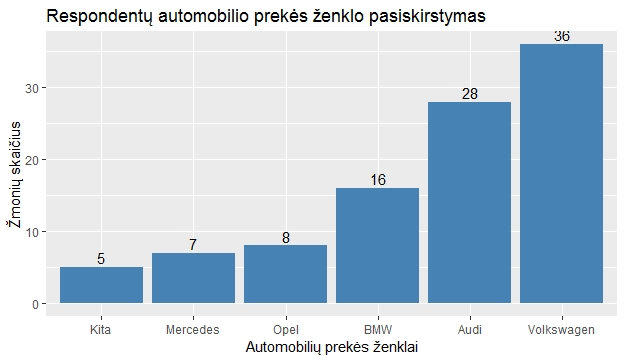
\includegraphics[scale=0.8]{plot1}
\end{figure}
 
Apaklausę respondentus, kurie turi savo automobilį, paaiškėjo tokie rezultatai.  Dauguma 36 proc. žmonių atsakė, kad turi „Volkswagen“ markės automobilį, 28 proc. respondentų naudojasi „Audi“ markės automobiliu, 16 proc. respondentai turi „BMW“ markės automobilį. 8 proc. respondentų atsakė, kad turi „Opel“  markės automobilį, 7 proc. respondentų priklausė „Mercedes“ prekės ženklui, o 5 proc. naudojasi kitu prekės ženklu. \\

\begin{table}[H]
\center
\begin{tabular}{|c|c|c|ll}
\cline{1-3}
Kriterijai                                                  & Žmonių skaičius & \begin{tabular}[c]{@{}c@{}}Procentinė\\   dalis (\%)\end{tabular} &  &  \\ \cline{1-3}
Kaina                                                       & 28              & 28                                                                &  &  \\ \cline{1-3}
\begin{tabular}[c]{@{}c@{}}Kaina ir\\   kokybė\end{tabular} & 22              & 22                                                                &  &  \\ \cline{1-3}
Prekės ženklas                                              & 39              & 39                                                                &  &  \\ \cline{1-3}
Kita                                                        & 11              & 11                                                                &  &  \\ \cline{1-3}
\end{tabular}
\caption{Kriterijai kaip respondentai renkasi prekę}
\label{tab:table3}
\end{table}

Atsižvelgiant į tai, kokie svarbiausi aspektai respondentams buvo perkant automobilį, informacija rodo, kad pirkėjo pirkimo sprendimas priklauso nuo šių faktorių : praeities patirtis, prekės ženklas, kokybė ir kaina. Dauguma respondentų 39 proc. pirkdami automobilį kreipia dėmesį į gerai žinomą prekės ženklą, 28 proc. respondentų manė, kad automobilio kaina yra svarbiausias faktorius perkant automobilį. Tačiau  22 proc pasissakė, kad tiek kokybė, tiek kaina yra svarbūs faktoriai. Be to, 11 proc. kreipia dėmesį į kitus aspektus (pvz.: automobilio dizainas)(\ref{tab:table3} lentelė) \\

\begin{figure}[H]
\center
\includegraphics[scale=0.8]{plot2}
\end{figure}

Tai labai įdomus klausimas apie respondentų požiūrį į mažesnius žinomus prekės ženklus. Respondentų buvo paklausta, ar jie domėjosi mažiau žinomais prekės ženklais. Nustatyta, kad 65 proc. respondentų atsakė „Ne“, o tai reiškia, kad respondentai dažniausiai domėjosi tik tais prekės ženklais, kurie yra žinomi. Taip pat nustatyta, jog 19 proc. respondentų vis dėlto domėjosi ir mažiau žinomais prekės ženklais , 16 proc. respondentų atsakė, jog domėjosi truputį, bet neperdaugiausiai. \\

Kokybės suvokimas tarp gerai žinomo prekės ženklo ir mažiau žinomų prekės ženklų - firminiai produktai turi geresnę kokybę. \\

\begin{table}[H]
\center
\begin{tabular}{|c|c|c|l}
\cline{1-3}
Atsakymas                                                      & Žmonių skaičius & \begin{tabular}[c]{@{}c@{}}Procentinė\\   dalis (\%)\end{tabular} &  \\ \cline{1-3}
Taip                                                           & 69              & 69                                                                &  \\ \cline{1-3}
Ne                                                             & 11              & 11                                                                &  \\ \cline{1-3}
\begin{tabular}[c]{@{}c@{}}Taip, bet\\   nevisada\end{tabular} & 20              & 20                                                                &  \\ \cline{1-3}
\end{tabular}
\caption{Žinomų prekės ženklų kokybė yra geresnė}
\label{tab:table4}
\end{table}

Kalbant apie žinomesnio prekės ženklo produkto kokybę įdomu tai, kad 
jie turi labai tvirtą asociaciją. Dauguma 69 proc.  atsakė „Taip“, jie mano, kad žinomesnių prekės ženklų produktai (šiuo atveju automobiliai) yra geresnės kokybės, 11 proc. respondentų atsakė, jog nesutinka su šiuo teiginiu, o 20 proc. respondentų mano, kad sutinka, tačiau taip yra nevisada. (\ref{tab:table4} lentelė)\\

\begin{figure}[H]
\center
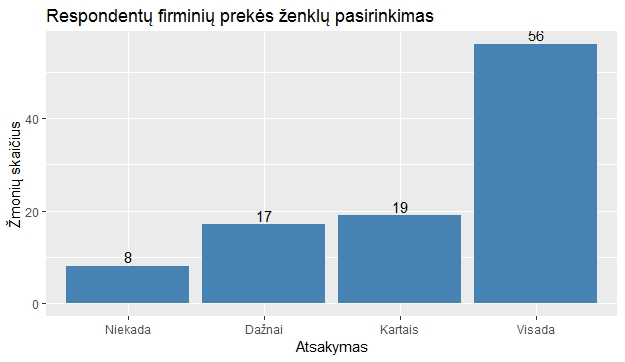
\includegraphics[scale=0.8]{plot3}
\end{figure}

Norėdama sužinoti, ar žmonės visada naudojasi firminiais produktais, respondentų buvo paklausta apie jų požiūrį į firminius produktus. Dauguma 56 proc. respondentų atsakė, kad jie visuomet renkasi firminius produktus. Kita vertus, 19 proc.  perka kartais, 17 proc. teigė, kad perka „dažnai“ ir 8 proc. atsakė „niekada“.  Rezultatas rodo, kad dauguma vartotojų pageidauja pirkti firminius produktus, nes tai simbolis kokybės, būklės ir patikimumo.

\justify
\section{Išvada}
\justify
\hspace{\parindent}
Šio straipsnio tikslas buvo sukurti gilesnį svarstymą apie prekės ženklo lojalumą.  Apklausa buvo atlikta tarp 100 respondentų, o duomenys atskleidė, kad prekės ženklas turi didelę įtaką pirkimo sprendimui. Iš tyrimo aišku, kad gerai žinomi firminiai automobiliai yra labiau žinomi tarp žmonių, nes vartotojai pasitiki prekės ženklu. Tai taip pat rodo, kad žmonės dažnai perka gerai žinomus prekės ženklo automobilius, nes jie žino apie prekės ženklo našumą arba galbūt jie jau buvo susidūrę su prekės ženklu ir turi gerą nuomonę apie jį. Pirkdamas tapatį prekės ženklą, pirkėjas tampa lojaliu tam prekės ženklui. Todėl gamintojas turi siūlyti aukščiausios kokybės paslaugas tam, kad patenkintų kliento lūkesčius. Taip pat prekės ženklo lojalumo stiprinimas tampa svarbia konkurencinio pranašumo įgijimo sąlyga įmonėms. Tačiau reikia pabrėžti, jog įmonės dar per mažai skiria tam dėmesio.
\justify

\newpage
\nocite{*}	
\printbibliography[title={Literatūra}]	

Aleliūnaitė, D., Urbanskienė, R. (2000). Prekės, jos ženklo ir vartotojų santykių reikšmė įmonės veiklai marketingo kultūros požiūriu // Inžinerinė ekonomika. Nr. 5 (10).\\

Lietuvos Respublikos prekių ženklų įstatymas. (2000). - \\
https://e-seimas.lrs.lt/portal/legalAct/lt/TAD/TAIS.111762?jfwid=tu0odnqqe


\end{document}



